% !Mode:: "TeX:UTF-8"
% 百分号表示注释。不会出现在最终论文中。
%% 请使用 XeLaTeX 编译本文. 更新目录、参考文献引用等要编译两次。
%\documentclass{HedaBachelor}
\documentclass[forprint]{HedaBachelor}
% 选项 forprint: 交付打印时使用, 避免彩色链接字迹打印偏淡. 注意:一般要求新的章开始于新的奇数页,所以在合适的地方已经设置好空白页,直接双面打印即可!无需更多设置。

\begin{document}
%%%%%%% 下面的内容主要自动产生封面, 据实修改{}中的内容.

%\miji{ }                      % 密级. 没有就空着.
\StudentNumber{20160123456789} % 填写自己的学号

\Year{2020}     %毕业年份
\title{河南大学本科毕业论文~\LaTeX~模板设计\\(改成你自己的论文题目)} % 自己的论文题目写入{}内,太长可以用"\\"换行,一般不超过25字。
\Etitle{A \LaTeX~Thesis Template for Henan University} % 英文题目
\author{令狐冲}                    % 作者名字
\Eauthor{LINGHU Chong}            %作者英文名
\Csupervisor{风清扬\quad 教~~授}        %指导教师中文名、职称.\quad表示空格
\Esupervisor{Prof.~Feng QingYang}     %指导教师英文名、职称
\Cmajor{测控技术与仪器}                  % 专业中文名
\Emajor{Instrumentation and Control Engineering}% 专业英文名
\Cschoolname{物理与电子学院}          % 学院名
\Eschoolname{School of Physics and Electronics} %学院英文名. 不确定的话, 请看一下自己学院的网页上是怎么写的. 别搞错了!
\date{2020年05月01日}                    % 日期, 要注意和英文日期一致!!
\Edate{May, 2020}                       % 英文封面日期

%-----------------------------------------------------------------------------
\pdfbookmark[0]{封面}{title}         % 封面页加到 pdf 书签
\maketitle
%\thispagestyle{empty}
\frontmatter
\pagenumbering{Roman}              % 正文之前的页码用大写罗马字母编号.
%-----------------------------------------------------------------------------
% !Mode:: "TeX:UTF-8"

%%% 此部分需要自行填写: (1) 中文摘要及关键词 (2) 英文摘要及关键词
%%%%%%%%%%%%%%%%%%%%%%%%%%%%%
%%% -------------  英文封面 (无需改动!!!)-------------   %%%
%%%%%%%%%%%%%%%%%%%%%%%%%%%%%
\thispagestyle{empty}
\renewcommand{\baselinestretch}{1.5}  %下文的行距
\vspace*{0.5cm}
\begin{center}
{\Large \bf BACHELOR'S DEGREE THESIS \\[1ex] OF HENAN UNIVERSITY }
\end{center}
\vspace{2.5cm}
\begin{center}{\zihao{2} \the\Etitle \par}\end{center}

\vfill

\begin{center}
\zihao{4}
\begin{tabular}{ r l }
 School:          & {\sc \the\Eschoolname}\\
  Major:          &   {\sc\the\Emajor}  \\
 Candidate:      &  {\sc \the\Eauthor}      \\
 Supervisor:     &  {\sc \the\Esupervisor}
\end{tabular}

\vspace*{2cm}
\begin{center}
   \ifprint % 文档打印, 使用黑白校徽.
  
\includegraphics[height=4cm]{hedalogo.pdf}       %%  黑白的.
  \else
  
\includegraphics[height=4cm]{hedalogo.pdf} %%  彩色的.
  \fi
\end{center}


\zihao{-2}
%\the\Schoolname\\
{\sc Henan University}

\vspace*{1.0cm}

\the\Edate

\end{center}
%%% 郑重声明部分无需改动

%%%---- 郑重声明 (无需改动!!!)------------------------------------%
%\newpage
%\vspace*{20pt}
%\begin{center}{\ziju{0.8}\textbf{\songti\zihao{2} 郑重声明}}\end{center}
%\par\vspace*{30pt}
%\renewcommand{\baselinestretch}{2}
%
%{\zihao{4}%
%
%本人呈交的学位论文, 是在导师的指导下, 独立进行研究工作所取得的成果,
%所有数据、图片资料真实可靠. 尽我所知, 除文中已经注明引用的内容外,
%本学位论文的研究成果不包含他人享有著作权的内容.
%对本论文所涉及的研究工作做出贡献的其他个人和集体,
%均已在文中以明确的方式标明. 本学位论文的知识产权归属于培养单位.\\[2cm]
%
%\hspace*{1cm}本人签名: $\underline{\hspace{3.5cm}}$
%\hspace{2cm}日期: $\underline{\hspace{3.5cm}}$\hfill\par}
%%------------------------------------------------------------------------------
%\baselineskip=23pt  % 正文行距为 23 磅
%%------------------------------------------------------------------------------
%



%%======中文摘要===========================%
\begin{cnabstract}
	%自己的论文摘要
摘要是论文内容不加注释和评论的简短陈述,应以第三人称陈述,采用“分析了……原因”、“认为……”、“对……进行了探讨”等记述方法进行描述。摘要是论文内容的高度概括,应具有独立性和自含性,即不阅读论文的全文,就能获得必要的信息。摘要应包括本论文的目的、主要研究内容和研究方法、研究结果及其理论与实际意义等,重点突出研究成果和结论。摘要中不宜使用公式、化学结构式、图表和非公知公用的符号与术语,不标注引用文献编号,同时避免将摘要写成目录式的内容介绍。摘要字数在300字左右。
关键词:关键词是为了文献索引工作从论文中选取出来用以表示全文主题内容信息的单词或术语。一般每篇论文应选取3~5个词作为关键词。关键词间用中文逗号分隔,最后1个词后不打标点符号。

\end{cnabstract}
\par
\vspace*{2em} %%产生空行

%%%%--  关键词 -----------------------------------------%%%%%%%%
%%%%-- 在下面的大括号中写入自己论文的关键词。注意: 每个关键词之间用“;”分开,最后一个关键词不打标点符号
\cnkeywords{毕业论文; \LaTeX{}; 模板  }

\cleardoublepage 

%%====英文摘要==========================%

\begin{enabstract}
This thesis is a study on the theory of \dots.

\end{enabstract}
\par
\vspace*{2em}

%%%%%-- Key words --------------------------------------%%%%%%%
%%%%-- 注意: 每个关键词之间用“;”分开,最后一个关键词不打标点符号
 \enkeywords{\LaTeX{}; XXX }
 \cleardoublepage 
 
    % 加入中英文摘要.中英文摘要请打开frontmatter.tex文档撰写。
%==========================把目录加入到书签,不用改动==============================%%%%%%
\pdfbookmark[0]{目录}{toc}
\tableofcontents

\mainmatter %% 以下是正文,开始写吧!
%%%%%%%%%%%%%%%%%%%%%%%%%%%--------main matter-------%%%%%%%%%%%%%%%%%%%%%%%%%%%%%%%%%%%%
\chapter{绪论}  %\chapter{章标题}
 Latex写论文是国际学术标准,省去了Word软件写论文的诸如格式排版、调整目录、页码格式、数学公式编号等等很多烦恼,能够让大家时间集中于论文内容的撰写,也能节省指导老师的宝贵时间,每年不用花太多时间修改论文格式,以便更好的指导论文。
 
 本文主要介绍和讨论了河南大学本科毕业论文的~\LaTeX~模板。
 指明了编译方法, 强调了公式排版的一些细节问题, 也指出了一些常见的排版错误。特别说明:本模板由高伟老师首次提出并在武汉大学模板的基础上修改而成,首先在指导的2020届学生中试用,暂时适用于物理与电子学院相关本科专业,其他学院和专业仅供参考。 
 
 \section{具体使用步骤} % \section{节标题}
本模板适用 TeX Live 软件环境. 建议安装最新版 TeX Live 2019 以及专用编辑器 TeXstudio. 

TeX Live 软件及编辑器TeXstudio安装及配置方法,百度很多,有个写的很详细参见网址:

\url{https://blog.csdn.net/zywhehe/article/details/83113214}

下面是使用步骤:
 \begin{description}

  \item[Step 1]  用专门的编辑器TeXstudio或者 WinEdt打开主文档 Bachelor--template.tex, 填写题目、作者等等信息, 书写正文.

  \item[Step 2]  最后,进入 includefile 文件夹,  打开 frontmatter.tex, backmatter.tex 这两个文档,  分别填写 (1) 中文摘要、英文摘要, (2) 致谢.

  \item[Step 3]  使用 XeLaTeX 编译. 具体见 \ref{sec-compile} 节.


\end{description}



\section{编译的方法}\label{sec-compile}

打开编辑器 TeXstudio "选项(options)"菜单,-> "设置 TeXstudio", ->弹出窗口中选中 "构建(Build)",->设置默认编译器为 xeletax. 
设置完毕。打开 Bachelor-template.tex 源文件按下 F5 键开始编译并预览生成的 PDF 文件。
更新目录、参考文献引用、公式引用等要编译两次。

若另存为新文档, 请确保文档保存类型为 \verb|:UTF-8|. 当然目前很多编辑器默认文字编码为 UTF-8.
编辑器TeXstudio或者 WinEdt 9.0之后的版本都是默认保存为 UTF-8 的. 

在PDF 文件中右键菜单可以跳转到 tex 源文件,在 tex 源文件中右键菜单同样可以跳转到PDF 文件对应位置。方便对比修改论文。


\section{文档类型选择}
文档类型有 2 种情形:

\begin{table}[ht]\centering \zihao{5}
\begin{tabular}{ll}
\hline
   \verb|\documentclass{HedaBachelor}|                     &  毕业论文 \\
   \verb|\documentclass[forprint]{HedaBachelor}|        &  毕业论文打印版 \\
\hline
\end{tabular}
\end{table}
相关解释见下节.


\section{打印的问题}
\begin{enumerate}[i)]
%  \item  论文要求\colorbox{yellow}{单面打印}.
  \item  关于文档选项 forprint: 交付打印时, 建议加上选项 forprint, 以消除编译生成的PDF文件中链接文字之彩色, 避免打印字迹偏淡.
  \item  注意:一般要求新的章开始于新的奇数页,所以在合适的地方已经设置好空白页,看到编译生成的pdf文件中的空白无页码页不用吃惊。直接双面打印即可!无需更多设置。
  \item  打印时留意不要缩小页面或居中. 即页面放缩方式应该是“无”(Adobe Reader XI 是选择“实际大小”).
           有可能页面放缩方式默认为``适合可打印区域'', 会导致打印为原页面大小的 $97\%$.
           文字不要居中打印, 是因为考虑到装订, 左侧的空白留得稍多一点(聪明的你一定发现偶数页是右侧空白稍多一点:-),本模板已作预留.
  \item  遗留问题: 封面已经尽量与河大教务处封面模板一致,可能仍然需要打印部重新制作.  校内打印部通常有现成的模板. 我们自己做的封面, 打印部不一定好用.
  \item	如果不是彩色打印机, 请在打印时, 选择将彩色打印为黑白, 否则彩色文字、图片打出的墨迹会偏淡.
\end{enumerate}


\textbf{问}: {\kaishu 生成 PDF 文件时,不能去掉目录和文章的引用彩色方框,请问怎么解决?}

\textbf{答}: {\kaishu 方框表示超级链接, 只在电脑上看得见. 实际打印时, 是没有的. 另外, 文档类型加选项 forprint 之后, 这些框框会隐掉的. }

 \vfill

本文档下载更新地址:
 \url{https://github.com/davidgao666/HedaBachelorTemplate}. 使用之前, 请移步查看是否有更新.

问题反馈及建议, 请联系: gaow@henu.edu.cn.



\chapter{杂七杂八的话}

\section{Readme}

模板文件的结构, 如下表所示:
 \begin{table}[ht]\centering \zihao{5}
\begin{tabular}{r|r|l}
	\hline\hline
	\multicolumn{2}{l|}{Bachelor-template.tex }       & 主文档. 在其中填写正文.             \\ \hline
	                                & frontmatter.tex & 中英文摘要.               \\ \cline{2-3}
	\raisebox{1em}{includefile 文件夹} &  backmatter.tex & 致谢.                       \\ \hline
	\multicolumn{2}{l|}{figures 文件夹}                  & 存放图片文件.                   \\ \hline
	\multicolumn{2}{l|}{HedaBachelor.cls }             & 定义文档格式的 class file. 不可删除. \\ \hline\hline
\end{tabular}
\end{table}

无需也不要改变、移动上述文档的位置.

\section{更新记录}
2019年11月28日更新:修订摘要页码问题,重新开始于罗马数字I.

2019年11月27日更新:修订中英文摘要页的格式,以符合河大教务处格式要求。正式上传到github网站。下载最新版地址为

\url{https://github.com/davidgao666/HedaBachelorTemplate}.

2019年11月26日更新:改定beta测试版。基于 TeXstudio 编辑器和texlive 2019 软件编译成功。主要是按照河南大学教务处及物理学院论文格式调整好了封面、章节标题样式;修订目录中三级标题字体分别为小四黑体、小四宋体和五号宋体;修订图、表标题的字号统一为五号;按照物理学院格式要求的顺序,把致谢调整到附录之后。实现无页码的空白页。

%2016 年 06 月更新: 正文字体为小四号; 英文字体为 Times New Roman; 修订图表标题的字体、字号; 修订目录的字号; 修订附录章节编号的问题. 
%                          非常感谢武汉大学数学与统计学院 2012 级张仕俊、林颖倩、宋俍辰等同学. 
%
%2016 年 05 月更新: 参考文献加到目录. 感谢武汉大学经济与管理学院的郑中天同学. [上次修订使用的版本有误, 非常抱歉.]
%
%2016 年 02 月更新: 调整为适应 TeX Live 2015 的版本.
%
%2014 年 06 月更新: 修改章节标题、声明标题、图表标题的字体和大小. 再次感谢孙启航同学.
%
%2014 年 05 月更新: 参考文献加到目录. 感谢武汉大学计算机学院孙启航同学、数学与统计学院李振坤同学指出这个纰漏.
%
%2013 年 12 月更新: 加上英文封面. 教务部的写作规范中的附例, 并没有英文封面. 但是遇到很多同学说要加上.

\section{段落与换行}

tex源文件中,空一行表示分段。

双斜线\\表示换行。是的,在编译生成的PDF论文中你看不到双斜线。关于latex的各种语法,各种不会的小问题,大家自行百度吧,或者仔细阅读本文档以及注释文字。

\section{数学公式}
latex语音强大功能之一就是敲公式。任何符号都可以敲出来。自动编号。看以下示例。

段落文字行中的公式,用两个美刀符号把公式语法代码包起来就行。如$\Delta=\sqrt{b^2-4ac}$. 还有:

独立成行带编号的公式,如标准二阶系统的闭环传递函数是下式\eqref{eq:erjiexitong}:

\begin{equation}\label{eq:erjiexitong}
\Phi(s)=\frac{\omega_n^2}{s^2+2\zeta \omega_n s+\omega_n^2}
\end{equation}
其中$\zeta$为阻尼系数,$\omega_n$为自然振动频率。

独立成行不编号的公式,如标准二阶系统的闭环频率特性是下式:

\begin{equation*}
\Phi(j\omega)=\frac{1}{(jT\omega)^2+2j\zeta T \omega+1}
\end{equation*}
其中$T=\frac{1}{\omega_n}$为时间常数。% 注意语法代码中的*表示不编号,不编号也就不能引用了,不需要加标签\label。

各种复杂公式的写法,还有各种特殊符号的语法命令,可以自己百度。

也可以从 MathType 等软件中敲好,再复制latex代码过来。

另外,推荐一个公式神器软件Mathpix snipping tool,只要截图就能识别公式,手写的公式都能识别,并自动生成latex源码。官网是 \url{https://mathpix.com/ }. 中文说明参见网址 
\url{https://blog.csdn.net/qq_34243930/article/details/89158366}.

\section{字体调节}
字体命令如下:

\begin{tabular}{ll}
	\hline %划一条横线
	命令             &  效果            \\
	\hline %划一条横线
	\verb|\songti|   & {\songti 宋体}   \\
	\verb|\heiti|    & {\heiti 黑体}    \\
	\verb|\fangsong| & {\fangsong 仿宋} \\
	\verb|\kaishu|   & {\kaishu 楷书}   \\
	\hline %划一条横线
\end{tabular}

\section{字号调节}
本模板已设置好大多数环境如标题、正文的字号大小和段落间距,基本不用调整。唯一要调整的是表格中的字号为五号字。参照以下字号命令: \verb|\zihao{}|   效果如下:\index{zihao}

\begin{tabular}{ll}
	\hline %划一条横线
    命令             &  效果            \\
	\hline %划一条横线
	\verb|\zihao{0}| &\zihao{0}  初号字 English \\
	\verb|\zihao{-0}|&\zihao{-0} 小初号 English \\
	\verb|\zihao{1} |&\zihao{1}  一号字 English \\
	\verb|\zihao{-1}|&\zihao{-1} 小一号 English \\
	\verb|\zihao{2} |&\zihao{2}  二号字 English \\
	\verb|\zihao{-2}|&\zihao{-2} 小二号 English \\
	\verb|\zihao{3} |&\zihao{3}  三号字 English \\
	\verb|\zihao{-3}|&\zihao{-3} 小三号 English \\
	\verb|\zihao{4} |&\zihao{4}  四号字 English \\
	\verb|\zihao{-4}|&\zihao{-4} 小四号 English \\
	\verb|\zihao{5} |&\zihao{5}  五号字 English \\
	\verb|\zihao{-5}|&\zihao{-5} 小五号 English \\
	\verb|\zihao{6} |&\zihao{6}  六号字 English \\
	\verb|\zihao{-6}|&\zihao{-6} 小六号 English \\
	\verb|\zihao{7} |&\zihao{7}  七号字 English \\
	\verb|\zihao{8} |&\zihao{8}  八号字 English \\
	\hline %划一条横线
\end{tabular}

\section{已加入的常用宏包}

宏包(package)是指latex平台实现各种神奇功能软件包。初学者不用考虑这一节内容,只管做好实验,编好实验程序,设计调试好电路,写论文就行了。模板已加入的有:

\begin{description}
%  \item[amsmath,amssymb]
  \item[cite]  参考文献引用, 得到形如 [3-7] 的样式.
  \item[color,xcolor]  支持彩色.
  \item[enumerate]  方便自由选择 enumerate 环境的编号方式. 比如

  \verb|\begin{enumerate}[(a)]| 得到形如 (a), (b), (c) 的编号.


  \verb|\begin{enumerate}[i)]| 得到形如 i), ii), iii) 的编号.

\end{description}

另外要说明的是,  itemize, enumerate, description 这三种 list 环境, 已经调节了其间距和缩进,
以符合中文书写的习惯.

\section{标点符号的问题}

建议使用半角的标点符号, 后边再键入一个空格. 特别是在英文书写中要注意此问题!

但是, 无论您偏向于全角或半角, 强烈建议您使用实心的句号, 只要您书写的是自然科学的文章.
原因可能是因为, 比如使用全角句号的句子结尾处的“$x$。”容易误为数学式~$x_0$(\verb|$x_0$|)吧.

以上是很多学术期刊杂志的要求,河大毕业论文并无此明确要求。正常用句号“。”就行。但是句子结尾是英文字母或数字时,最好用半角的实心标点符号。如 xyz.

\section{引用的问题}


\subsection{参考文献的引用}

参考文献的引用, 用命令~\verb|\cite{ }|. 大括号内要填入的字串, 是自命名的文献条目名.

比如, 通常我们会说:

 {\kaishu
关于此问题, 请参见文献 \cite{r2}. 作者某某还提到了某某概念\upcite{r1}.}


上文使用的源文件为:

 {\kaishu
关于此问题, 请参见文献~\verb|\cite{r2}|. 作者某某还提到了某某概念~\verb|\upcite{r1}|.
}

其中~\verb|\upcite| 是自定义命令, 使文献引用呈现为\CJKunderdot{上标形式}.

({\heiti 注意:} {\kaishu 这里文献的引用, 有时需要以上标形式出现, 有时需要作为正文文字出现, 为什么?})

另外, 要得到形如~\cite{r1,r3,r4,r5} 的参考文献连续引用, 需要用到 cite 宏包(模板已经加入),
在正文中使用~\verb|\cite{r1,r3,r4,r5}| 的引用形式即可.
或者, 连续引用的上标形式: 使用~\verb|\upcite{r1,r2,r3}|, 得到\upcite{r1,r2,r3}.

\subsection{定理和公式的引用}

\begin{theorem}[谁发现的]\label{th-abcd}
最大的正整数是~$1$.
\end{theorem}

\begin{proof}
要找到这个最大的正整数, 我们设最大的正整数为~$x$, 则~$x \geqslant 1$, 两边同时乘以~$x$, 得到
\begin{equation}\label{eq-abc}
x^2 \geqslant x.
\end{equation}
而~$x$ 是最大的正整数, 由~\eqref{eq-abc} 式得到
\[
x^2 = x.
\]
所以
\begin{equation*}
x = 1.
\end{equation*}
\end{proof}

定理~\ref{th-abcd} 是一个重大的发现.

%%%%----- 定义等环境的举例 --------
\begin{definition}[整数]
 正整数(例如 1, 2, 3)、负整数(例如 ${−1}$, $−2$, $−3$)与零(0)合起来统称为{\heiti 整数}.
\end{definition}

\begin{remark}
  整数集合在数学上通常表示为 $\mathbf{Z}$ 或 $\mathbb{Z}$, 该记号源于德语单词 Zahlen(意为``数'')的首字母.
\end{remark}

\begin{proposition}
任意两个整数相加、相减、相乘的结果, 仍然是整数.
\end{proposition}

\begin{example}
  $1+2=3$.
\end{example}

\begin{corollary}
   在整数集合内, 相加、相减、相乘运算是封闭的.
\end{corollary}

\section{图形与表格}

支持对~eps, pdf, jpg, png等等常见图形格式.

再次\colorbox{red!45}{澄清一个误会}: \LaTeX{} 支持的图形格式绝非 eps 这一种. 无需特意把图片转化为 eps.

用形如~\verb|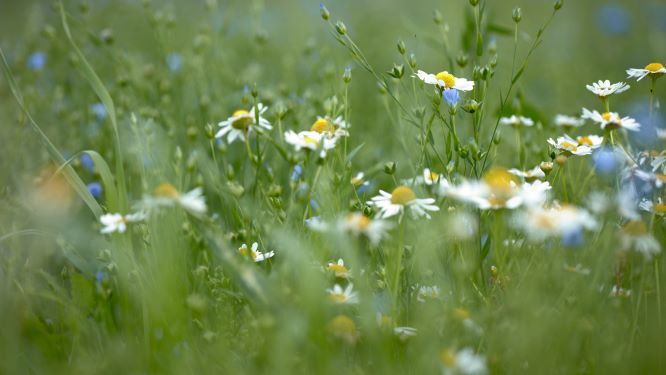
\includegraphics[width=12cm]{Daisy.jpg}| 的命令可以插入图片. 选项[width]用来调整图片宽度,其数值可以用绝对值12cm,也可以用相对于行宽度的数值。图片高度会等比例自动缩放。比如:

\verb|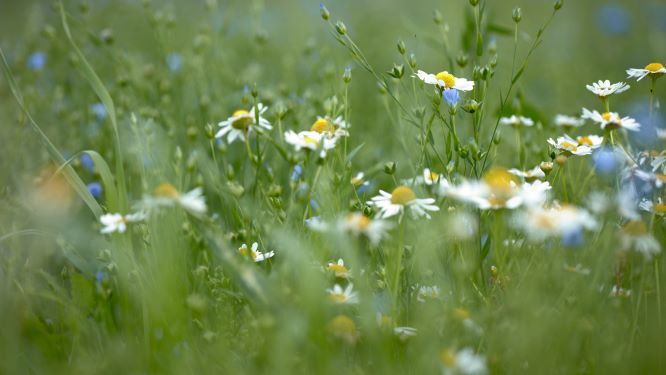
\includegraphics[width=0.9\textwidth]{Daisy.jpg}|. 

如图~\ref{fig:1} 是一个纳入~jpg 图片的例子. 所有图片应放在本模板文件所在的文件夹中figures文件夹中。

%插入已有图片代码示例如下:

\begin{figure}[!htb]
\centering
  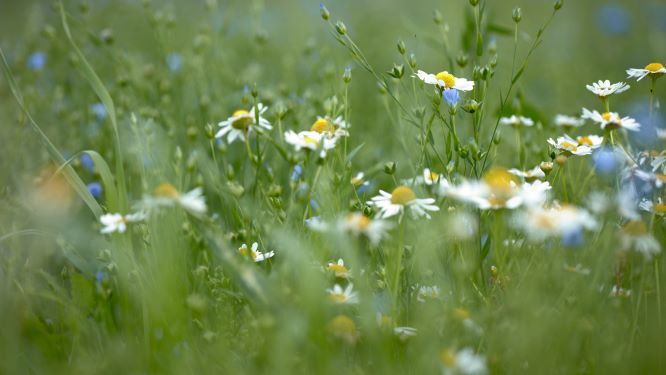
\includegraphics[width=\textwidth]{Daisy.jpg}
  \caption{一个彩色 jpg 图片的例子}
  \label{fig:1}
\end{figure}

表格问题, 建议使用“三线表”, 表中内容字号要调整为5号字。如下表 \ref{tab:1}示例.

%绘制并插入表格代码如下:
\begin{table}[ht]
\centering %%居中
\zihao{5}  %%5号字 
\caption{一般三线表示例}
\vspace{-0.8em}  %%减小表题与表格间距
\label{tab:1}
    \begin{tabular}{c c c c c c c c c c c}
    \hline
    123 & 4  & 5  & 123 & 4 & 5123 & 4 & 5 & 123 & 4 & 5\\
    \hline
    67 & 890 & 13 & 123 & 4 & 5123 & 4 & 5 & 123 & 4 & 5\\
    67 & 890 & 13 & 123 & 4 & 5123 & 4 & 5 & 123 & 4 & 5\\
    67 & 890 & 13 & 123 & 4 & 5123 & 4 & 5 & 123 & 4 & 5\\
    \hline
    \end{tabular}
\end{table}



%%%%============================================================================================================%%%

\chapter{其他事项}

\section{广告时间}
以下是广告时间, 插播一段广告:
\begin{itemize}
    \item 程序流程图的制作, 可以用MicroSoft Visio 软件绘制,存成pdf格式或者JPG格式。另外,\LaTeX 平台可以用 pgf, 也叫 tikz.
          pgf 的长处是源文件直接植入~\TeX~文档, 管理起来非常方便.
    这里有武汉大学黄正华老师写的一个关于初次使用~pgf~的帖子:\\    \url{http://bbs.ctex.org/forum.php?mod=viewthread&tid=30480}.(已经打不开了,大家自己百度)
    \item 生成参考文献, 建议使用~BibTeX.\index{BibTeX} 这里有武汉大学黄正华老师写的一个文档: \\
    \url{http://bbs.ctex.org/forum.php?mod=viewthread&tid=26056}.(已经打不开了,大家自己百度)

          {\kaishu 使用 BibTeX{} 做参考文献时,
      借助 EndNote 或者 NoteExpress, 还有Mendeley,都可以非常漂亮简单地解决 bib 文件的录入问题.
      当然 EndNote 本身就是 Thomson Corporation 推出的(和 SCI 搜索引擎是同一家公司), 和多个重要文献搜索引擎有良好的功能配合.

      Google 学术搜索也提供了文献的 bib 格式.
      录入参考文献时, 偶尔用一用 Google 学术搜索, 还可以核查或减少录入的错误, 并减少录入的工作量.}

    \item \LaTeX 也可进行幻灯片\index{幻灯片}的制作, 建议使用~Beamer Package. 网上可以找到很多模板。这里有武汉大学黄正华老师写的一个模板, 谨供参考:\\
    \url{http://bbs.ctex.org/forum.php?mod=viewthread&tid=27695}.(已经打不开了,大家自己百度)
\end{itemize}

\section{参考文献格式问题}

请大家仔细阅读文件《河南大学教务处本科生毕业论文格式规范》和 《河南大学物理与电子学院-学士学位论文撰写规范》中关于文献列表的格式说明和范例。

\chapter{实验结果与分析}

\section{实验方法}

\subsection{硬件平台}

\subsection{软件平台}

\section{实验结果}
\subsection{结果1}

\subsection{结果1分析}

\chapter*{结~~~~论} %星号*表示没有章编号,波浪号表示空一格
\addcontentsline{toc}{chapter}{结论} %%加入目录和PDF书签中,勿改。

学位论文的结论作为论文正文的最后一章单独排写,不加章标题序号,不标注引用文献。

结论应是作者在学位论文研究过程中所取得成果的概要总结,不能与摘要混为一谈。结论的撰写应符合以下基本要求:
\begin{enumerate}
	\item 结论具有相对的独立性,不应是对论文中各章小结的简单重复。结论要与绪论相呼应,总结全文,加深题意,以自身的条理性、明确性、客观性反映论文价值。
	\item 结论措辞要准确、严谨,不能模棱两可,避免使用“大概”、“或许”、“可能是”等词语。结论中不应有解释性词语,而应直接给出结果。结论中不应叙述自己学习、生活等与论文无关的内容。
	\item 结论应指出论文研究工作的局限性或遗留问题,如条件所限,或存在例外情况,或本论文尚难以解释或解决的问题。
	\item 常识性的结果或重复他人的结果不应作为结论。
\end{enumerate}
%%%============================================================================================================%%%

%%%=== 参考文献 ========%%%
\cleardoublepage\phantomsection
\addcontentsline{toc}{chapter}{参考文献}
\begin{thebibliography}{00}

  \bibitem{r1} 作者. 文章题目 [J].  期刊名, 出版年份,卷号(期数): 起止页码.

  \bibitem{r2} 作者. 书名 [M]. 版次. 出版地:出版单位,出版年份:起止页码.

  \bibitem{r3} 邓建松等, 《\LaTeXe~科技排版指南》[M], 科学出版社.

  \bibitem{r4} 吴凌云, 《CTeX~FAQ (常见问题集)》, \textit{Version~0.4}, June 21, 2004.

  \bibitem{r5} Herbert Vo\ss, Mathmode, \url{http://www.tex.ac.uk/ctan/info/math/voss/mathmode/Mathmode.pdf}.


\end{thebibliography}


%%%-------------- 附录. 不需要可以删除.-----------
\appendix

\chapter{测试}

\section{第一个测试}
测试公式编号
\begin{equation}
1+1=2.
\end{equation}

表格编号测试

\begin{table}[h] 
  \centering
  \caption{测试表格}
  \begin{tabular}{*{20}c}
     \hline
     % after \\: \hline or \cline{col1-col2} \cline{col3-col4} ...
     11 & 13  & 13  & 13  & 13 \\
     12 & 14  & 13  & 13  & 13 \\
     \hline
   \end{tabular}
\end{table}


%\chapter{附录测试}
%
%测试
%
%\chapter{附录测试}
%
%测试


%%%-------------- 致谢. 不需要可以删除.-----------
% !Mode:: "TeX:UTF-8"
%%%%%%%%%%%%%%%%%%%%%%%%%%%%-------致谢--------%%%%%%%%%%%%%%%%%%%%%%%%%%%%%%%%

\acknowledgement
\addcontentsline{toc}{chapter}{致谢} %%加入目录和PDF书签中,勿改。


%本部分内容非必要,学校学院也没有要求。不建议写。

感谢你, 感谢他和她, 感谢大家。

特别感谢武汉大学论文模板作者数学院黄正华老师!


致谢属于非必须内容,可以不写。







 %%%致谢,可以删除本行

\cleardoublepage   %%勿删
\end{document}     %%勿删



